\chapter{Introduction}
\label{Chapter:intro} 

This chapter provides the reader with an understanding of the research context, the significance of the study, the research problem/question, \& an outline of the structure of the thesis. The following  should be included in this chapter:

\begin{enumerate}

\item Research Background and Context:

	\begin{itemize}
	\item Provide an overview of the broader research area and its significance. Explain why this field is important and how your research fits into it.
	\item Mention key developments, theories, or studies related to your topic.
	 Highlight any gaps, unresolved questions, or limitations in the existing literature that your research aims to address.
   	\end{itemize}

\item Research Problem or Question:
	\begin{itemize}	
	\item Clearly state the specific research problem or question that your thesis addresses. This should be concise and to the point.
	\item Explain the relevance and importance of the research problem and its potential impact on the field.
   \end{itemize}

\item Research Objectives and Hypotheses:
	\begin{itemize}	
	\item Outline the objectives of your research. What are you trying to achieve or investigate?
	\item If applicable, state any hypotheses that you intend to test or assumptions you are making in your research.
	   \end{itemize}

\item Research Scope and Limitations:
	\begin{itemize}	
	\item  Define the boundaries of your research. What will be included and excluded from your study?
	\item Discuss any practical or methodological limitations that might affect the research.
	   \end{itemize}

\item Research Significance and Contributions:
	\begin{itemize}	
	\item Describe the potential contributions of your research to the field. What new knowledge, insights, or applications will your work offer?
	\item Explain how your research builds upon or extends existing work.
	   \end{itemize}

\item Thesis Structure:
	\begin{itemize}	
	\item Provide an overview of the organization and structure of the thesis. Mention how the subsequent chapters are connected and the purpose of each chapter.
	   \end{itemize}

\item Methodological Approach (optional):
	\begin{itemize}	
	\item If your research involves a unique or complex methodology, you can briefly introduce it in the introduction. However, detailed methodological explanations are often placed in a separate chapter.
	   \end{itemize}

\item Justification for the Study:
	\begin{itemize}	
	\item Explain why your research is relevant not only from an academic standpoint but also in terms of practical applications or societal impact.
	   \end{itemize}

\item Motivation and Personal Connection (optional):
	\begin{itemize}	
	\item Some introductions include a personal motivation or connection to the research topic. This can provide a human touch and explain why you, as the researcher, are passionate about the subject.
   \end{itemize}

\end{enumerate}

The introduction chapter should be well-structured, engaging, and clear. It should set the stage for the rest of the thesis, helping readers understand the purpose of the research and why it matters.

\begin{quote}
Think about who will read this thesis? \newline
Think about why they would want to read your thesis?
\end{quote}



\section{Research Question}  

Research questions guide research activities where the method, theory and results articulate findings in these activities.
Some characteristics of research quesitons are: 
1. Clarity and Specificity; 
1. Feasibility;
3. Relevance;
4. Originality; 
5. Testability;
6. Significance and
7. Open-Endedness.

\begin{quote}
\rqs{1}:~ Research Question 
\end{quote}

\begin{quote}
\rqs{2}:~ Research Question 
\end{quote}

\begin{quote}
\rqs{2}.A:~ Research Question \newline
\rqs{2}.B:~ Research Question 
\end{quote}
 
 

   
\subsection{Headings, Depth-Level, Table and Figure}

\begin{enumerate}
\item Depth level upto 3 is preferred. That is, chapter, section and subsection. Anything further makes it difficult to follow. There are no rules for this.  

\item Table:~\ref{table:connectingpapersrq} is an example of a table. 

\item Citations and reference example: \cite{salvendy2012handbook} and \cite{salvendy1994design}.

\item Figure:~\ref{fig:chapteroutline} is a picture of a two arm robot that might change the world \cite{abb2017}.


\end{enumerate}	
 

\begin{table}[t]
\centering
\caption{ Example of a table.}
\begin{tabularx}{.950\linewidth}{cXXXXXX}
\toprule
& \multicolumn{6}{c}{ Appended Articles}\\
\cline{2-7}
    RQ           						&  \Rmnum{1}		& \Rmnum{2} 	&	\Rmnum{3} &	\Rmnum{4} &	\Rmnum{5} 			&	\Rmnum{6}	 		\\ 
\cline{2-7} %

             \rqs{1}        		& \checkmark			&    	 					&	 \checkmark   &	\checkmark  &	\checkmark 		&	 \checkmark     		\\              
             \rqs{2}.A        		&  					   		& \checkmark 	&	 \checkmark &	\checkmark  	&	\checkmark 		&	 									  	\\ 
             \rqs{2}.B      		&  								& \checkmark 	&  \checkmark  &	 \checkmark  &	\checkmark  &		 						    	 	\\ 
\bottomrule
\end{tabularx}
\label{table:connectingpapersrq} 
\end{table}



 
\begin{figure}[h]
  	\centering
               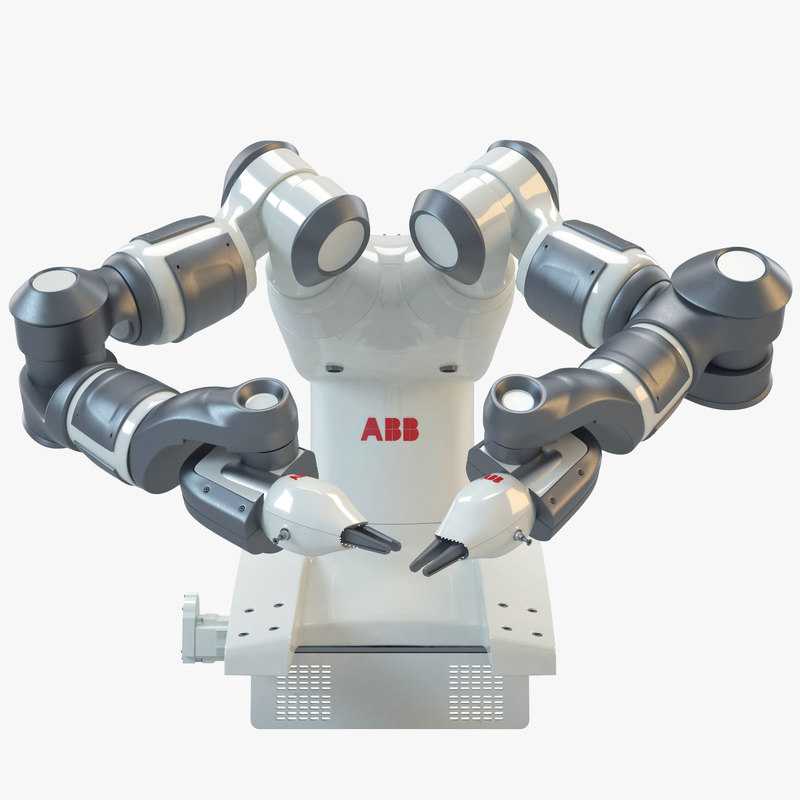
\includegraphics[width=7.0cm]{./gfx/yumi}
               \caption{Picture of a Collaborative Robot \cite{abb2017}.}
               \label{fig:chapteroutline}
\end{figure}

 